\documentclass[a4paper]{article}
%% Seitenaufbau
\usepackage[top=3cm, bottom=2.5cm, left=3.5cm, right=3.5cm]{geometry}

%% Schriftbild
\usepackage{lmodern}  % Latin Modern Zeichensatz
\usepackage[utf8]{inputenc}  % Unterstuetzung von Umlauten im Quelltext
\usepackage[T1]{fontenc}  % Korrekte Umlaute im Output
\usepackage[ngerman]{babel}  % Silbentrennung nach neuer Rechtschreibung
\renewcommand{\familydefault}{\sfdefault}  % Serifenlose Schrift
\usepackage{setspace}\onehalfspacing  % 1.5-facher Zeilenabstand
\renewcommand{\arraystretch}{1.5}  % 1.5-facher Zeilenabstand (Tabellen)
\setlength{\parindent}{0pt}  % Keine Einrueckung am Beginng von Absaetzen
\sloppy  % Weniger strikte Silbentrennung

%% Literaturverzeichnis (BibTex)
\usepackage{natbib}
\bibliographystyle{apalike} % Layout des Literaturverzeichnisses

%% Verlinkung von Inhaltsverzeichnis, Bildern und Formeln
\usepackage[pagebackref,linktoc=page]{hyperref}  % Verlinkung von URLs und Referenzen
\usepackage{color}  % Definition von Linkfarben
\definecolor{DarkRed}{rgb}{0.5,0,0}
\hypersetup{
  colorlinks,
  citecolor=DarkRed,
  linkcolor=DarkRed,
  urlcolor=blue}

%% Mathematikumgebung
\usepackage{mathtools}
\usepackage{amssymb}  % Erweiterte Bibliothek mathematischer Symbole
% \usepackage{euler}  % Serifenlose Schrift in Formelumgebungen
% \renewcommand{\deg}{\ensuremath{^{\circ}}}  % Grad Zeichen im Text
% \renewcommand{\epsilon}{\varepsilon}  % Nutze "richtiges" Epsilon

%% Grafikumgebungen
\usepackage{graphicx}  % Erweiterte Grafikumgebung
\usepackage{float}  % Automatische Positionierung von Bildern

% %% Formeln, Bilder und Tabellen pro section nummerieren
% \numberwithin{equation}{section}
% \numberwithin{figure}{section}
% \numberwithin{table}{section}

%% Blindtext zum Testen des Layouts
\usepackage{blindtext}

%% Inhalt der Titelseite
\title{Versuch 0: Beispielprotokoll}
\author{Gruppe X\\Max Mustermann\\Erika Mustermann}
\date{\today\\Geomatikum, Raum 1536a}

%%%%%%%%%%%%%%%%%%%%%%%%%%%%%%%%%%%%%%%%%%%%%%%%%%%%%%%%%%%%%%%%%%%%%%
\begin{document}
\maketitle
\thispagestyle{empty}\newpage
\thispagestyle{empty}\newpage
\tableofcontents
\newpage

\section{Exponentialfunktion}
Gleichung~\ref{eq:efunktion} beschreibt eine Exponentialfunktion. Der Verlauf
der Funktion hängt zusätzlich zu $x$ von einem Parameter $\tau$ ab.

\begin{equation}\label{eq:efunktion}
y = e^{\frac{-x}{\tau}}
\end{equation}

Abbildung~\ref{fig:efunktion} zeigt den Verlauf der Funktion für drei
verschiedene Werte von $\tau$.

\begin{figure}[ht]
  \centering
  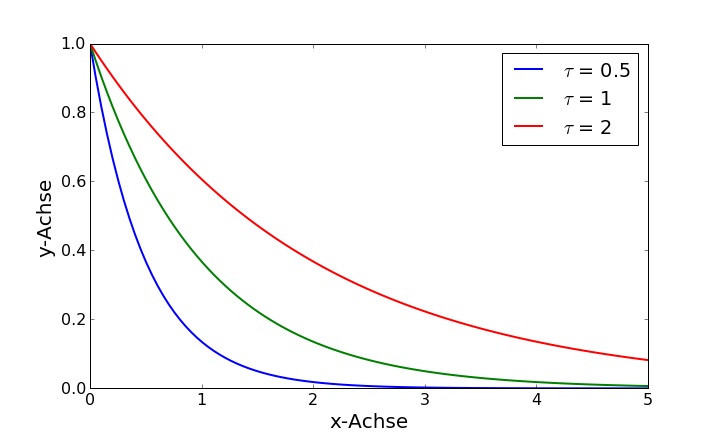
\includegraphics[width=\textwidth]{plot.png}
  \caption{Verlauf der Exponentialfunktion für verschiedene $\tau$.}
  \label{fig:efunktion}
\end{figure}

Eine Übersicht der Funktionswerte für die verschiedenen Kurven in Abbildung
\ref{fig:efunktion} kann aus Tabelle~\ref{tab:funktionswerte} entnommen werden.

\begin{table}[ht]
  \centering
  \caption{Funktionswerte von y für verschiedene $\tau$.}
  \begin{tabular}{|c|c|c|c|}\hline
  $x$ & $\tau =0.5$ & $\tau=1$ & $\tau=2$\\\hline
  0 & 1.000000 & 1.000000 & 1.000000\\\hline
  1 & 0.135335 & 0.367879 & 0.606531\\\hline
  2 & 0.018316 & 0.135335 & 0.367879\\\hline
  3 & 0.002479 & 0.049787 & 0.223130\\\hline
  4 & 0.000335 & 0.018316 & 0.135335\\\hline
  5 & 0.000045 & 0.006738 & 0.082085\\\hline
  \end{tabular}
  \label{tab:funktionswerte}
\end{table}

BibTex bietet eine einfache Möglichkeit eine Literaturliste zu verwalten um
beispielsweise auf das Praktikumsskript \citep{IPrak2016} zu verweisen.

Auf den folgenden Seiten erscheint einiger Blindtext, um das Layout
vollbeschriebener Seiten darzustellen.
\blinddocument
\blindmathpaper

% BibTex-Literaturverzeichnis (Pfad ohne Dateiendung angeben)
\bibliography{literatur}
% Literatur dem Inhaltsverzeichnis hinzufügen
\addcontentsline{toc}{section}{Literatur}

\end{document}
